\documentclass[letterpaper, 11pt]{article}
\usepackage {graphicx}
\usepackage{multicol}
\usepackage{hyperref}
\usepackage{geometry}
\geometry{margin=3cm}
\title{	

Genome Wide Association Study using Espresso Methods
}

\author{ Janis Waser}
\begin{document}
\maketitle




\section{Goal}
\label{sec:goal}
Genome wide association studies  (GWAS) is increasingly reliable and thus able to explain biological phenomena. A polygenic risk score is easily computable, but only gives limited insight to the inner mechanisms which are involved. Analyzing all possible combinations by brute-force for large data sets is not feasible and we must find methods which circumvent this complexity and still produce reliable results.

We are using a minimal cover algorithms to find a small selections of single nucleotide polymorphisms (SNPs) in a causal relationship for a given binary phenotype.  With these selections, we would like to explain the phenotypes.  Further, we investigate the genome-wide spanning relations between SNPs and potential groupings of the phenotype such as different subtypes of a disease. 


\tableofcontents
\newpage
\section {Quality control}
We want to emphasize the importance of quality control (QC) for this approach as it relies heavily on the assumption that the data has no inconsistencies. 

Our data stems from a GWAS/PRS tutorial and the corresponding Git directory which we also use for quality control \cite{tutorial}. It has 109 subjects and 1'073'226 SNPs after the aforementioned QC.  \\



For the selection of approaches the number of permitted unknowns is crucial, which is set to 2\% per individual and SNP. In the scope this means that there might still exist above 20'000 unknowns per individual. 
\section{Espresso}
Espresso is a tool that performs 2-level logic minimisation. It uses heuristics to find a satisfying minimal cover. It takes a logic table as input and outputs a minimized circuit.  The output is not guaranteed to be optimal. \\

"-" can used as don't cares. It is possible to specify special input types such as  \emph{.type fr} to indicate that not in case of an underspecified truth tables the underspecified cases are treated as don't cares. 


\section{Translation of genetic data into binary}
\label{sec:encode}
Most genetic data is stored in two pairwise inherited strings this is true particular for human autosomal genes. The manifestation can be made up from one of the four nucleobases (A/C/G/T) or an indentation of any length or a deletion (non-existence). The information for any particular SNP might also be partially missing. For any given position there commonly exist two different manifestations, one is labelled as the no-risk allele and the other allele is referred to as risk allele. There is no consensus for every SNP on what allele should be considered the risk allele, generally the variant with lower sampling rates is considered the risk allele. Two different studies might find different might find different risk alleles but they would still agree on the same manifestation which is in correlation with the disease. \\


We abstract the manifestations to a count of the occurrences of the risk allele. This count we decode into two digits long binary number. To avoid the unnecessary big Hamming distance of 2 between the counts of 2 ($10_2$) and 1 ($01_2$), while the smaller distance between 2 and 0 ($00_2$) would only have a Hamming distance of 1, we encode 2 as $11_2$. For the effect of this choice consider Figure \ref{fig:binary}.\\

Phenotypes for each individual should already exist in an easily binary translatable form.  We focus on binary phenotypes, if this approach shows promising results it is also possible to extend the approach to continuous  data or different potentially related diseases with pleiotropy. 

\section{Evaluation of results}
\label{sec:evaluate}
We use a range of different criteria to approximate the quality of our method. Each criteria has its own advantages and flaws which should always be taken into consideration. No single criteria is sufficient for showing a working method rather does it give an indication.
\begin{enumerate}
\item Previous identification of SNPs by other researchers
\item Out of data prediction accuracy of the phenotype
\item PRS 
\item Products 
\item Literals
\item Time and complexity of the solution\end{enumerate}

We might also discuss potential issues or perks of a specific method which go beyond this list. 
\section{ Tried methods}
\subsection{Primitive approaches}
\subsubsection{Entire}
Taking the entire dataset and let it be solved by Espresso, is impossible as the time requirements grow exponentially, as we know the problem is not even in P. 
\subsubsection{Omitting parts of the dataset}
Taking partial parts of the dataset and never discovering other parts is possible though it is highly doubtful how a good solution should found consistently. For discovering the dataset and experimenting this we did run some experiments. In the context of this experiment when we refer to $n$ we mean the amount of SNPs. 

\begin{enumerate} 
\setcounter{enumi}{1}
\item The out-of-data prediction accuracy is as predicted around the 50\% mark, potentially slightly above for hign $n$. 
\setcounter{enumi}{3}
\item High $n$ yield a smaller product, we explain deviations from this rule by the diverging paths taken in Espresso or in case of different dataset by the difference of possibilities. 
\item Same as for products, just more pronounced as in practice this are higher numbers and therefore more possible outcomes(events). 
\item This analysis is fast and easy to execute for small n, it scales exponentially with n. 
\end{enumerate}


The following table gives an overview of the acquired results with all 109 subjects considered. Each SNP is decoded as two digits, hence the input size is double the amount of selected SNPs. The results are averaged, estimated and depend on the selection of the SNPs and are used as a baseline assumption:

\begin{center}
\begin{tabular}{ c| c| c| c}
 \textbf{Input size (2n)} & \textbf{Products} & \textbf{Literals} & \textbf{Time} \\ \hline
 $<$120& -&-&$<$ 1s\\
 200 & 50 & 3-6&5s\\  
 400 & 40 & 2-4  & 10s \\
 1000& 30&2-3&40s\\
 2000&25&2&8min
\end{tabular}
\end{center}

If there are less than 60 SNP, it is generally not possible to find an assignment as the truth table would be over-specified. \\

A random selection of SNP generally decreases the identified products required for a minimal cover, this trends also affects the literals but is less pronounced. Additionally, it was discovered that missing data is not distributed equally among the data and therefore in sequential analysis even for a relative high n it might not be possible to find a cover due to over-specification. For random selections this constitutes less of a concern as we are guaranteed to have at most 2\% missingness.  
\begin{figure}[h]
\centering{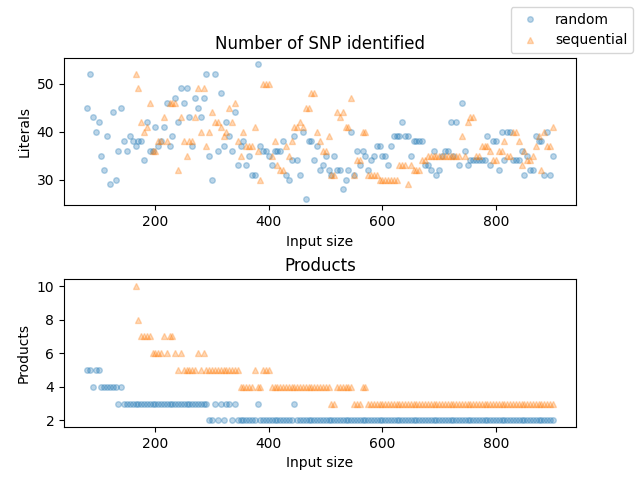
\includegraphics[width=\linewidth]{randseq} \caption {Comparison between random and sequential selection methods }
}
\end{figure}

The random method will be used exclusively in all future analysis. \\


Different encoding methods also influence the result. The adjusted method is selected going forwards (see \ref{sec:encode})

\begin{figure} \centering{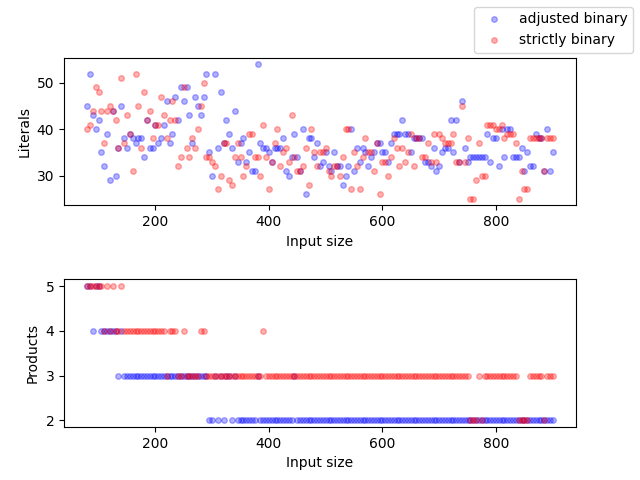
\includegraphics[width=\linewidth]{binarycomp} 
\caption {Comparison between different binary encoding methods }\label{fig:binary}
}

\end{figure}

The adjusted method will be used exclusively in all future analysis. 

\subsubsection{Iterative approaches}

\subsection{Pyramid scheme}
\subsection{Subgroup scheme}


\begin{thebibliography}{99}
\bibitem{tutorial}
\emph{Marees AT et al. } A tutorial on conducting genome-wide association studies: Quality control and statistical analysis. \url{https://pmc.ncbi.nlm.nih.gov/articles/PMC6001694/}

\end{thebibliography}
\end{document}